%%%%%%%%%%%%%%%%%%%%%%%%%%%
% Author : Paul Gaborit (2009)
% under Creative Commons attribution license.
% Title : Pascal's triangle and Sierpinski triangle
% Note : 17 lines maximum
\documentclass[border=2mm, tikz]{standalone}
%\usepackage[landscape,margin=1cm]{geometry}
%\pagestyle{empty}
%\usepackage[T1]{fontenc}
%\usepackage{lmodern}

\usepackage{tikz}
\usetikzlibrary{positioning,shadows,backgrounds,shapes.geometric}
\begin{document}
\centering

%
% x=\sqrt{3/4}*minimum size
% y=3/4*minimum size
%
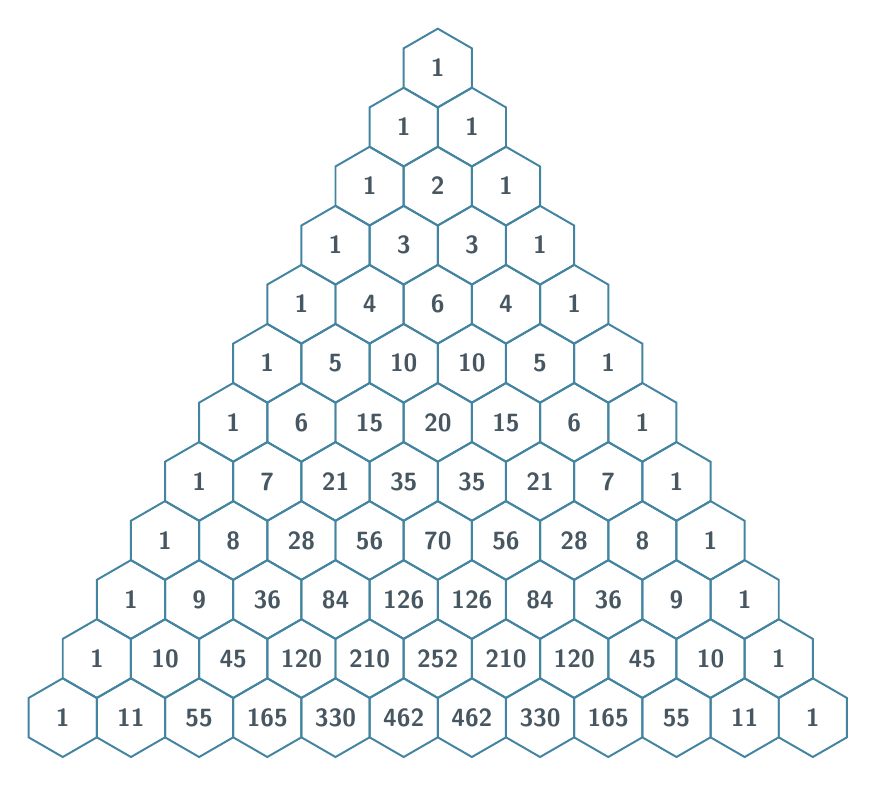
\begin{tikzpicture}[y=7.5mm,x=8.66mm]
  % some colors
  \colorlet{even}{cyan!60!black}
  \colorlet{odd}{orange!100!black}
  \colorlet{links}{red!70!black}
  \colorlet{back}{yellow!20!white}
  % some styles
  \tikzset{
    box/.style={
      regular polygon,
      regular polygon sides=6,
      minimum size=10mm,
      inner sep=0mm,
      outer sep=0mm,
      text centered,
      font=\small\bfseries\sffamily,
      text=#1!50!black,
      draw=#1,
      line width=.25mm,
      rotate=30,
    },
    link/.style={black,  shorten >=2mm, shorten <=2mm, line width=1mm},
  }
  % Pascal's triangle
  % row #0 => value is 1
  \node[box=even] (p-0-0) at (0,0) {\rotatebox{-30}{1}};
  \foreach \row in {1,...,11} {
     % col #0 =&gt; value is 1
    \node[box=even] (p-\row-0) at (-\row/2,-\row) {\rotatebox{-30}{1}};
    \pgfmathsetmacro{\myvalue}{1};
    \foreach \col in {1,...,\row} {
      % iterative formula : val = precval * (row-col+1)/col
      % (+ 0.5 to bypass rounding errors)
      \pgfmathtruncatemacro{\myvalue}{\myvalue*((\row-\col+1)/\col)+0.5};
      \global\let\myvalue=\myvalue
      % position of each value
      \coordinate (pos) at (-\row/2+\col,-\row);
      % odd color for odd value and even color for even value
      \pgfmathtruncatemacro{\rest}{mod(\myvalue,2)}
       \node[box=even] (p-\row-\col) at (pos) {\rotatebox{-30}{\myvalue}};
    }
  }
  
  
%   \begin{pgfonlayer}{background}
%     \foreach \i/\j in {4/1,5/1,5/2,6/2,7/6,8/6,8/7,9/7}
%         \node[box=even,fill=odd]  at (p-\i-\j) {};
%   \end{pgfonlayer}

    % \draw[link] (p-4-1.center)--(p-6-2.center);
    % \draw[link] (p-5-1.center)--(p-5-2.center);
    % \draw[link] (p-7-6.center)--(p-9-7.center);
    % \draw[link] (p-8-6.center)--(p-8-7.center);
    % \node[right=5mm of p-8-8.center, align=left]  {$(36-7)+(28-8)=49$};
    % \node[left=5mm of p-5-0.center, align=right]  {$(15-4)+(10-5)=16$};

\end{tikzpicture}

\end{document}